\section{Chapter 1}

\subsection{Donald Hebb} 
Organization of behaviour - 1949 learning mechanism:
\begin{itemize}
	\item When an axon of cell A is near enough to excite a cell B and repeatedly or persistently takes part in firing it, some growth process or metabolic change takes place in one or both cells such that A's efficiency, as on of the cells firing B, is increased.
	\item As A repeatedly excites B, its ability to excite B improves.
	\item Neuron that fire together wire together.
\end{itemize}

\subsection{Hebbian Learning}
\begin{itemize}
	\item If neuron $x$ repeatedly triggers neuron y, the synaptic knob connecting $x$ to $y$ get larger.
	\item In mathematical model:
	\[ w_{xy} = w_{xy} + \eta xy \]
	\item Weight of the connection from input neuron $x$ to output neuron $y$.
	\item This simple formula is actually the basis of many learning algorithms in machine learning.
\end{itemize}

This idea however is fundamentally unstable:
\begin{itemize}
	\item Stringer connections will enforce themselves.
	\item No notion of "competition".
	\item No \textit{reduction} in weights.
	\item Learning is unbounded.p
\end{itemize}

People came up with all kinds of modifications for it to try to make it more stable:
\begin{itemize}
	\item Allowing for weight normalization.
	\item Forgetting
\end{itemize}
This lead to the Generalized Hebbian learning, aka Sanger's rule where the contribution of input is \textit{incrementally distributed} over multiple outputs.
\[ w_{ij} = w_{ij} + \eta y_j\left( x_i -	\sum_{k=1}^{j}	w_{ik}y_k																									\right) \]

\subsection{A better model}
Frank Rosenblatt
\begin{itemize}
	\item Psychologist, Logician
	\item Inventor of the solution to everything, aka Perceptron
\end{itemize}

\paragraph{Original perceptron model}
Consider the eye structure:
\begin{itemize}
	\item Groups of sensors on retina combine into cells in association in the \textbf{projection area}.
	\item Groups of \textbf{projection area} combine into Association cells in \textbf{association area}.
	\item Signals from \textbf{association area} cells combine into response cell \textbf{R}.
	\item All connections may be excitatory or inhibitory.
\end{itemize}

Rosenblatt's perception model can then be further simplified:
\paragraph{Simplified perceptron model}

\begin{figure}[h]
	\centering
	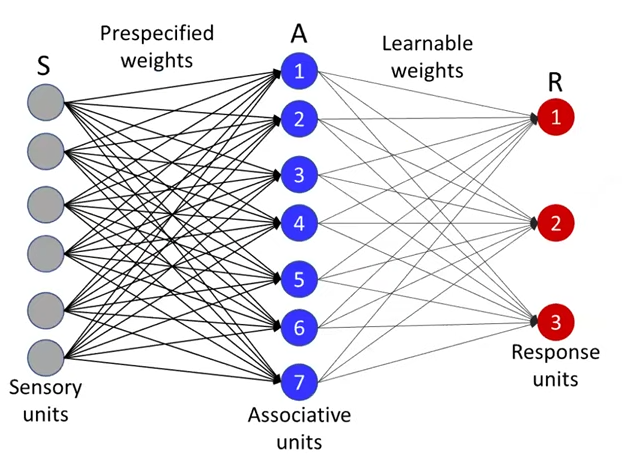
\includegraphics[scale=0.5]{simplified_perceptron_model}
\end{figure}

\begin{itemize}
	\item Association units commbine sensory input with fixed weights.
	\item Response units combine associative units with learnable weights.
\end{itemize}

Each of the units can be perceived as shown below:
\begin{figure}[h]
	\centering
	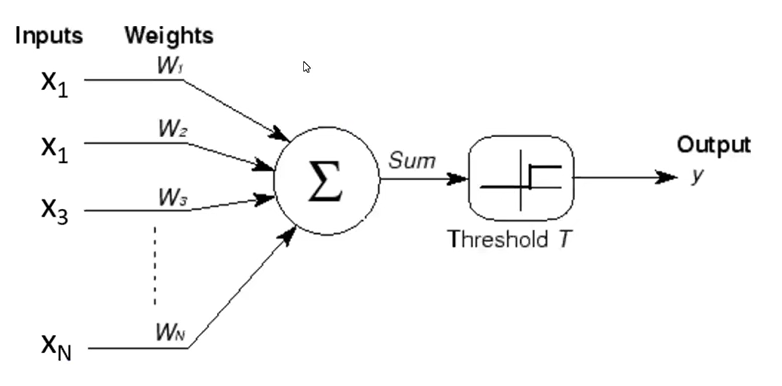
\includegraphics[scale=0.5]{perceptron_fbd}
\end{figure}

\begin{itemize}
	\item Number of inputs combine linearly.
	\item Threshold logic is applied at the output of the unit: It will only fire if the weighted sum of the input exceeds threshold.
\end{itemize}

\[ 
Y = 
\begin{cases} 
	1, & \text{if } \sum_{i}w_ix_i - T \geq 0 \\
	0, & \text{else }
\end{cases}
\]

\subsection{The Universal Model}
Originally assumed could represent any Boolean circuit and perform any logic. However this was not true and this cause the research in neural networks died down because of the overhype. However, Rosenblatt was right, he not only gave us basic model, he also gives us the learning algorithm.

\[ \mathbf{w} = \mathbf{w} + \eta (d(\mathbf{x}) - y(\mathbf{x}))\mathbf{x} \]

Sequential learning:
\begin{itemize}
	\item $d(\mathbf{x})$ is the desired output in response to input $\mathbf{x}$.
	\item $y(\mathbf{x})$ is the actual output in response to $\mathbf{x}$.
	\item Weight parameter is changed when the actual response of the neuron does not match the desired response of the neuron.
	\item If the actual response of the neuron exceeds the desired response of the neeuron, then the weight will decrease.
	\item If the actual response is lesser than the desired response, the weight will increase.
\end{itemize}

\paragraph{Single perceptron is not enough}
While this model able to mimic boolean logic such as AND, OR and NOT, it is not capable to mimic XOR gate. This imply that individual elements are weak computational elements and networked elements are required. However, with multilayered perceptron, XOR gate can be constructed:
\begin{itemize}
	\item Start with two inputs, A and B.
	\item Use AND gate to compute A and NOT B.
	\item Use another AND gate to compute NOT A AND B.
	\item Use an OR gate to combine the outputs of thee two AND gate.
\end{itemize}

This would lead to construction of perception network to represent a much more generic model:
\begin{itemize}
	\item Perceptrons can be multi-layered.
	\item Can compose arbitrarily complicated boolean functions.
	\item In cognitive terms, it should be capable to compute arbitrary boolean functions over sensory input.
\end{itemize}

\subsection{Difference between brain and neural networks}
\begin{itemize}
	\item Brains have real inputs.
	\item We are capable to make non-Boolean inferences and prediction.
\end{itemize}

\begin{figure}[h]
	\centering
	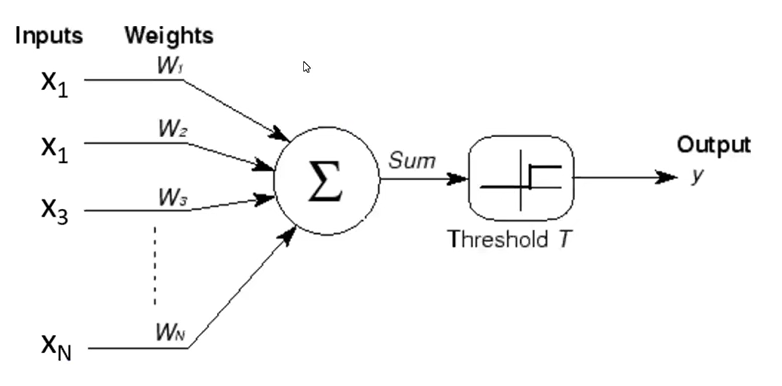
\includegraphics[scale=0.5]{perceptron_fbd}
\end{figure}

\noindent We can however try to implement \textbf{real inputs} on the perceptron model:
\begin{itemize}
	\item $x_1,x_2,...,x_N$ are real-valued.
	\item $w_1,w_2,...,w_N$ are real-valued.
	\item Unit is only fired if weighted sum of input matches or exceeds the threshold values $T$.
\end{itemize}

\begin{equation}
Y = 
\begin{cases} 
	1, & \text{if } \sum_{i}w_ix_i - T \geq 0 \\
	0, & \text{else }
\end{cases}
\end{equation}

\hfill\break
This create a boundary condition such that $\sum w_ix_i = T$ where every sum of inputs that's greater than $T$ will fire and everything that is less than $T$ would not fire.

\hfill\break
That being said, this provides an alternative view:
\begin{itemize}
	\item The neuron has a threshold \textbf{activation function} $\theta (z)$ operates on the weighted sum of inputs plus a bias. (Affine function of the inputs).
	\item The boundary $b$, is the value such that the affine term is equal to zero.
	\item Linear function is an affine function that passed through origin.
	\item $\theta (z)$ outputs a $1$ if $z$ is non-negative $0$ otherwise.
	\item Unit fires if weighted input matches or exceed threshold.
\end{itemize}
\[ 
y = \theta \left( \sum_{i}w_ix_i + b 																								\right)
\]

\[ 
\theta(z) = 
\begin{cases} 
	1, & \text{if } z \geq 0 \\
	0, & \text{else }
\end{cases}
\]

\hfill\break
On real numbers, this equation produce a hyperplane such with line separation of $w_1x_1 + w_2x_2 + ... + w_nx_n = T$ where one side of the plane is $1$ and the other side of the plane is $0$. This would means that a perceptron that operates on real-valued vectors is a type of linear classifier.

\begin{figure}[H]
	\centering
	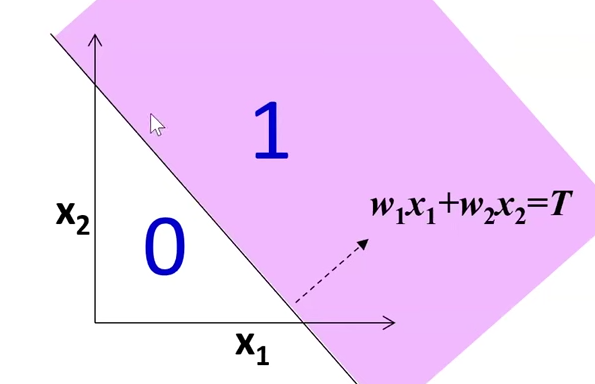
\includegraphics[scale=0.5]{hyperplane}
\end{figure}

\hfill\break
Similarly, for two-dimensional inputs, if we ever to plot the function, the function is going to looks like a step function. On one side, the output is $1$ and on the other side, the output is $0$.

\begin{figure}[H]
	\centering
	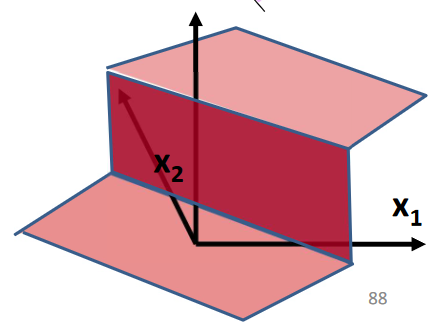
\includegraphics[scale=0.5]{2d_hyperplane}
\end{figure}

\hfill\break
Once we can see how the perceptron model works, we can finally see how it performs Boolean's functions.

\begin{figure}[H]
	\centering
	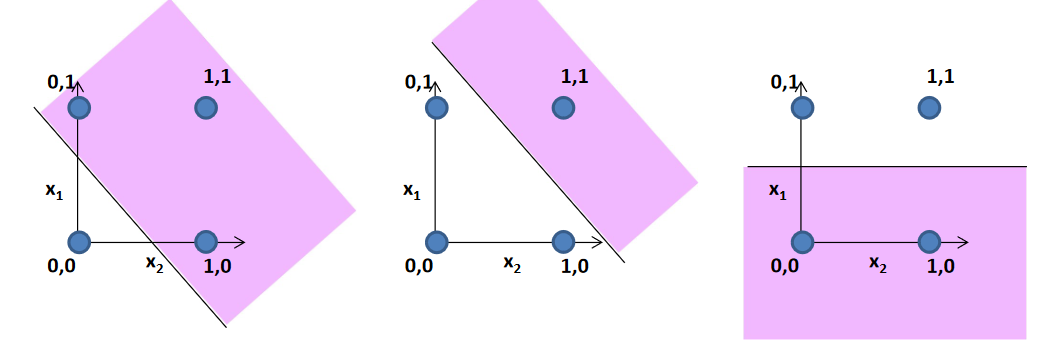
\includegraphics[scale=0.5]{1_boolean}
\end{figure}

\hfill\break
That being said, Boolean's perceptron is also linear classifiers:
\begin{itemize}
	\item Purple regions have output of $1$ in the figures.
	\item The left figure showcase OR-function.
	\item The middle figure showcase AND-function.
	\item The right figure showcase NOT-function.
	\item This is also the reason why a simple perceptron model is not enough to compose XOR-function.
\end{itemize}

\subsection{Perceptron as basic logic gates.}

\paragraph{AND Gate}
From our knowledge of logic fates, we know that an AND logic table is given by the diagram below.

\begin{flushleft}
	\begin{table}[H]
	\centering
	\begin{tabular}{|c|c|c|}
		\hline
		$x_1$ & $x_2$ & y \\
		\hline
		$0$ & $0$ & $0$   \\
		$0$ & $1$ & $0$   \\
		$1$ & $0$ & $0$   \\
		$1$ & $1$ & $1$   \\
		\hline
	\end{tabular}
\end{table}
\end{flushleft}

\hfill\linebreak
In order to interpret weights and bias to construct AND perceptron, we first need to understand that the output of an AND gate is $1$ only if both inputs (in this case $x_1$ and $x_2$) are $1$. Following the steps listed above:

From 
\begin{align}
	w_1\times x_1 + w_2\times x_2 + b
\end{align}

Initializing $w_1$, $w_2$, as $1$ and $b$ as -1, we get:
\begin{align}
	x_1(1) + x_2(1) - 1
\end{align}

Passing the first row of the AND logic table, ($x_1 = 0, x_2 = 0$), we get:
\begin{align}
	0 + 0 - 1 = -1
\end{align}

From the perceptron rule, if $\mathbf{w}x + b \leq 0$, then $y=0$, therefore this row is correct. Repeating the same process for each of the row:
\begin{align*}
	0 + 0 - 1 &= -1 \\
	0 + 1 - 1 &= 0 \\
	1 + 0 - 1 &= 0 \\
	1 + 1 - 1 &= 1 \\
\end{align*}

Therefore, we can conclude that in order for the perceptron to be able to model AND gate, the perceptron algorithm is:
\begin{align}
	x_1 + x_2 - 1
\end{align}

\begin{figure}[H]
	\centering
	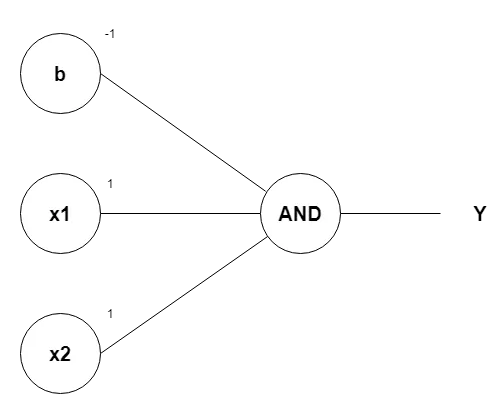
\includegraphics[width=0.5\textwidth]{2_and_gate}
\end{figure}

\paragraph{OR Gate}

\begin{flushleft}
	\begin{table}[H]
		\centering
		\begin{tabular}{|c|c|c|}
			\hline
			$x_1$ & $x_2$ & y \\
			\hline
			$0$ & $0$ & $0$   \\
			$0$ & $1$ & $1$   \\
			$1$ & $0$ & $1$   \\
			$1$ & $1$ & $1$   \\
			\hline
		\end{tabular}
	\end{table}
\end{flushleft}

From 
\begin{align}
	w_1\times x_1 + w_2\times x_2 + b
\end{align}

Initializing $w_1$, $w_2$, as $2$ and $b$ as -1, we get:
\begin{align}
	x_1(2) + x_2(2) - 1
\end{align}

Passing the first row of the OR logic table, ($x_1 = 0, x_2 = 0$), we get:
\begin{align}
	0 + 0 - 1 = -1
\end{align}

From the perceptron rule, if $\mathbf{w}x + b \leq 0$, then $y=0$, therefore this row is correct. Repeating the same process for each of the row:
\begin{align*}
	0 + 0 - 1 &= -1 \\
	0 + 2 - 1 &= 1 \\
	1 + 2 - 1 &= 2 \\
	2 + 2 - 1 &= 3 \\
\end{align*}

Therefore, we can conclude that in order for the perceptron to be able to model OR gate, the perceptron algorithm is:
\begin{align}
	2x_1 + 2x_2 - 1
\end{align}

\begin{figure}[H]
	\centering
	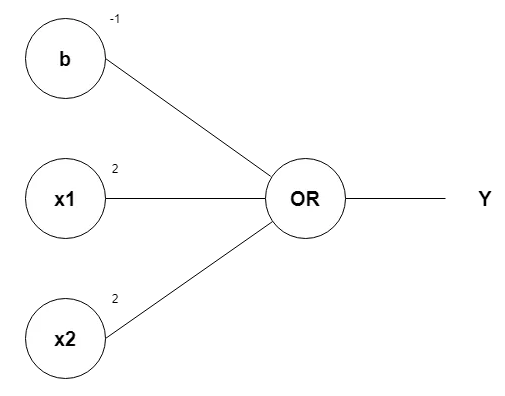
\includegraphics[width=0.5\textwidth]{2_or_gate}
\end{figure}

\paragraph{NOT Gate}

\begin{flushleft}
	\begin{table}[H]
		\centering
		\begin{tabular}{|c|c|}
			\hline
			$w$  & y \\
			\hline
			$0$ & $1$    \\
			$1$ & $0$    \\
			\hline
		\end{tabular}
	\end{table}
\end{flushleft}

From the diagram, the output of NOT gate is the inverse of the input. Since $w_2$ does not exists, the remaining equation would be:

\begin{align}
	w_1\times x_1 + b
\end{align}

Initializing $w_1$, as $-1$ and $b$ as 1, we get:
\begin{align}
	x_1(-1) + 1
\end{align}

Passing the first row of the NOT logic table, ($x_1 = 0$), we get:
\begin{align}
	0 + 1 = 1
\end{align}

Passing the second row of the NOT logic table, ($x_1 = 1$), we get:
\begin{align}
	-1 + 1 = 0
\end{align}

Therefore, we can conclude that in order for the perceptron to be able to model NOT gate, the perceptron algorithm is:
\begin{align}
	-x_1 + 1
\end{align}

\begin{figure}[H]
	\centering
	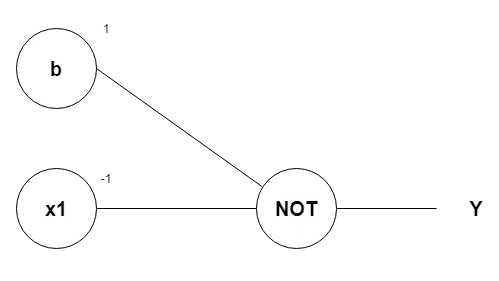
\includegraphics[width=0.5\textwidth]{2_not_gate}
\end{figure}


\hfill\break
We are able compose complicated decision boundaries by combining multiple linear perceptron by building a network of units with single output that firees if the input is in the desired regions. For example, we can use 5 perceptron model to compose 5 boundary condition of a pentagon. For each perceptron, the network will fire if the input is in the yellow area.

\begin{figure}[H]
	\centering
	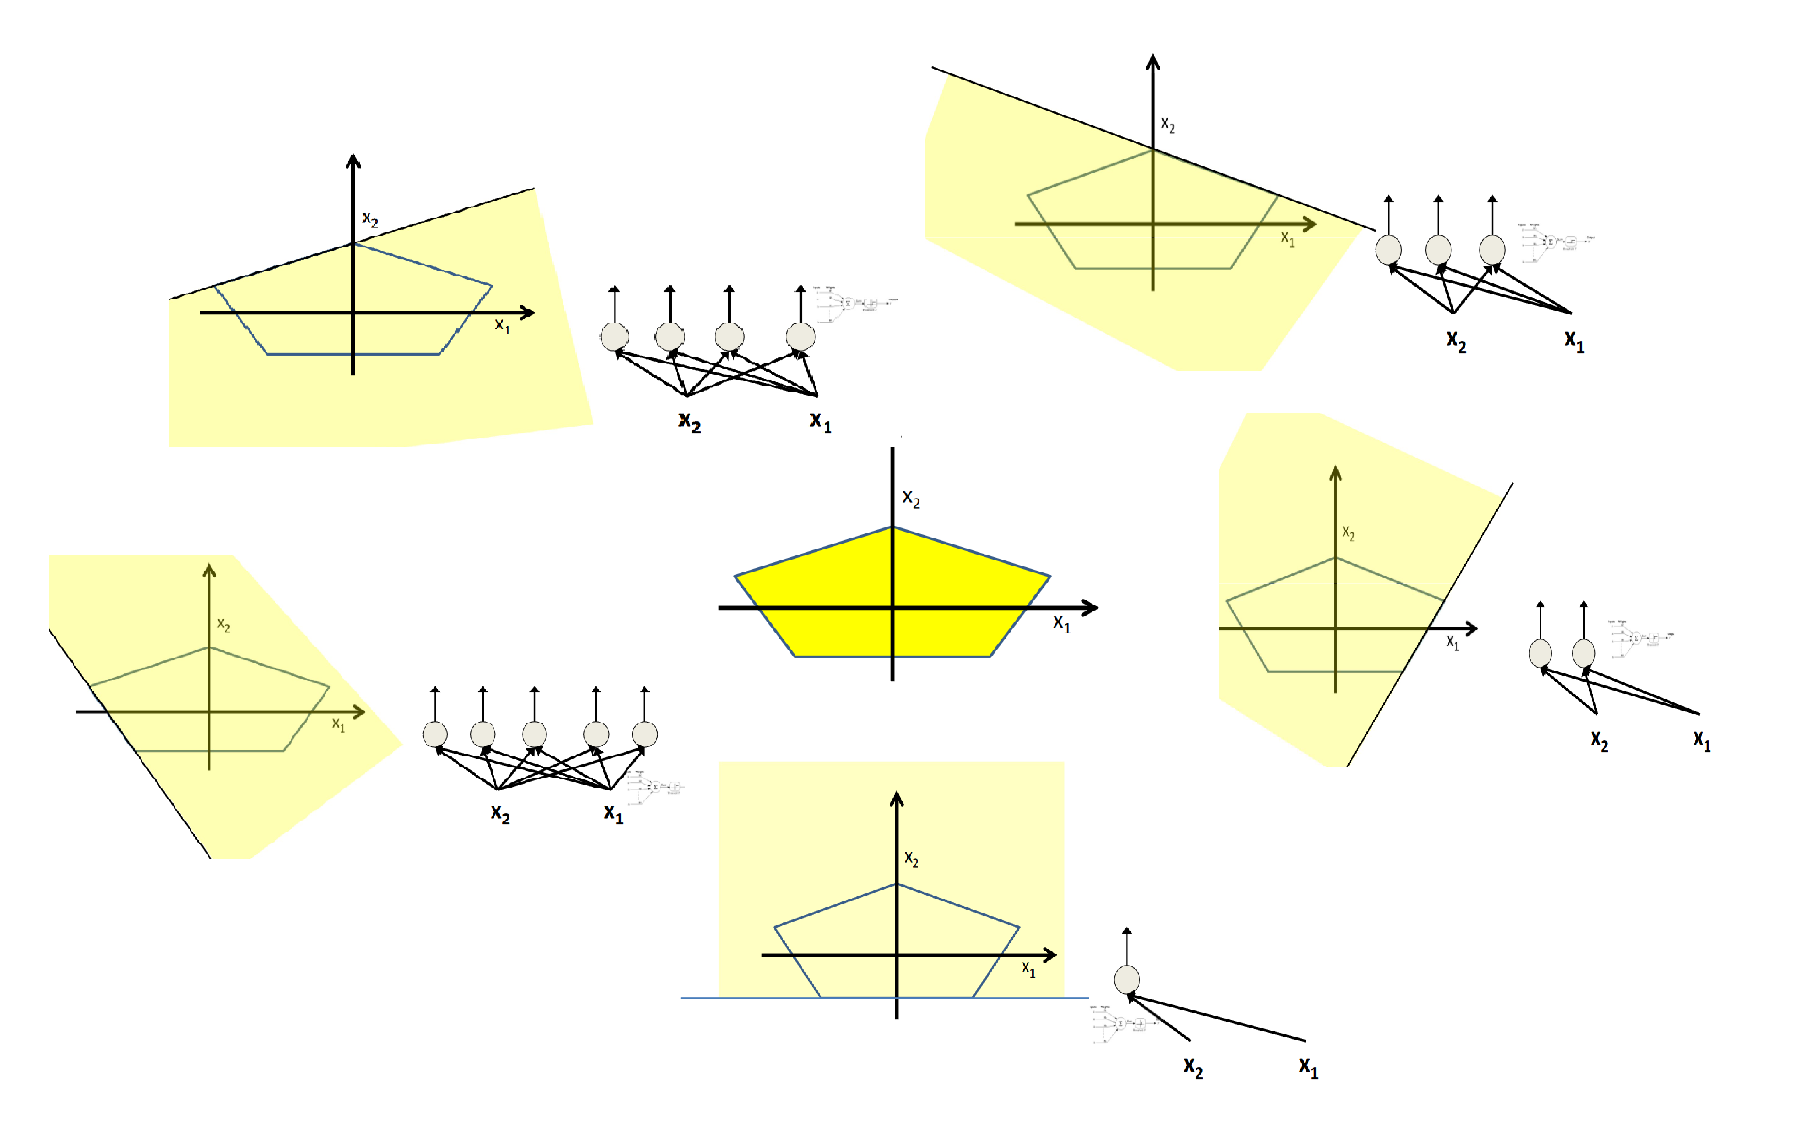
\includegraphics[width=\textwidth]{1_multi_model_perceptron}
\end{figure}

\hfill\break
Given this perceptrons, we can AND them together capture the pentagon decision boundary.

\begin{figure}[H]
	\centering
	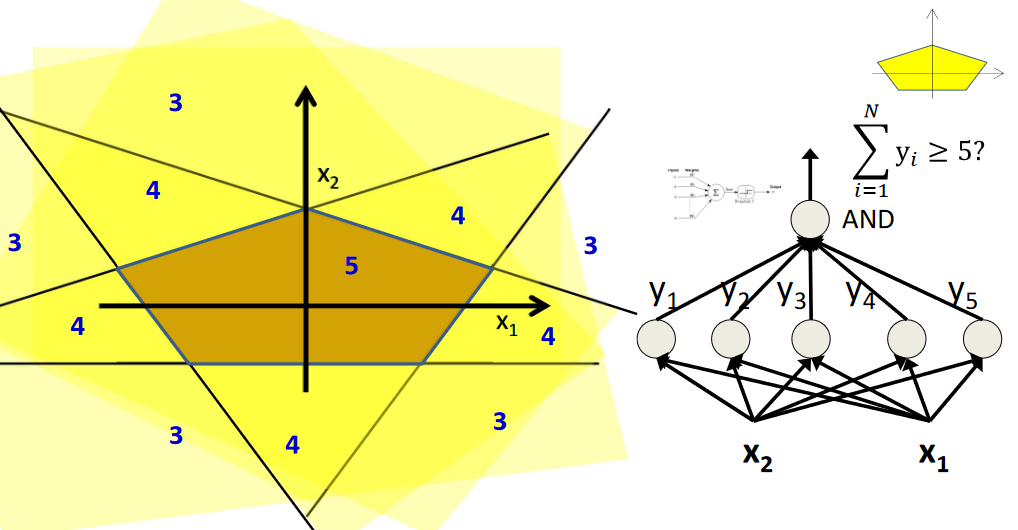
\includegraphics[width=\textwidth]{1_pentagon}
\end{figure}

\hfill\break
This also imply that much more complex boundary condition can be solved as well.

\begin{figure}[H]
	\centering
	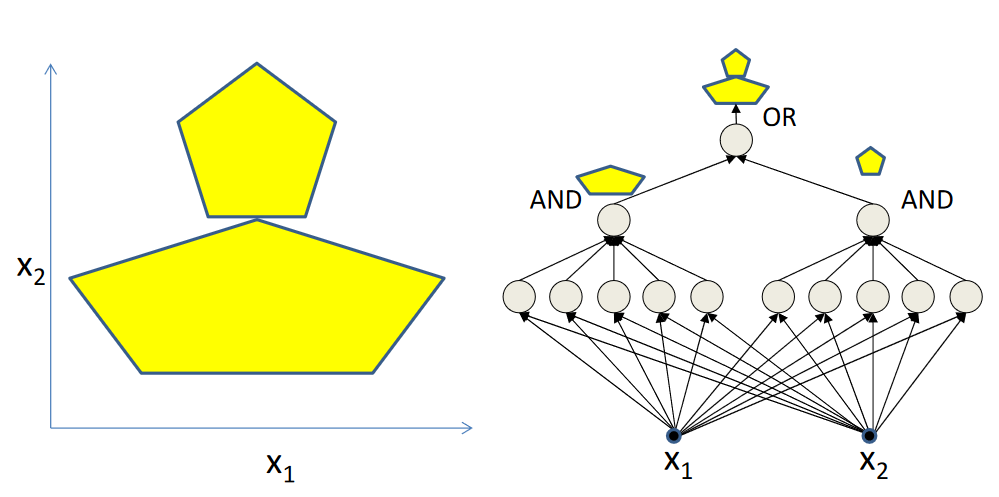
\includegraphics[width=\textwidth]{1_complex}
\end{figure}

\hfill\break
The network will fire if the input is in the yellow area:
\begin{itemize}
	\item "OR" two polygons
	\item This would means that a third layer of perceptron that behaves as "OR" gate is required.
\end{itemize}

\hfill\break
As the multi-layered perceptron is capable to solve complex decision boundaries, it can be used to solve:
\begin{itemize}
	\item Classification problems - finding decision boundaries in high-dimensional space.
	\item For example, the MNIST dataset every image as at least 784 dimensions boundary that need to be solved.
	\item MLP can be considered as universal classifiers as for any decision boundary, we can construct MLP that captures it with arbitrary precision.
\end{itemize}

\subsection{Continuous Valued Outputs}
So far we have covered networks which have Boolean functions where the inputs were Boolean and the output was Boolean. We also discussed functions that took continuous valueed inputs that gave Boolean or categorical output. This section covers the possibility of the networks having real-valued inputs with continuous valued output.

\hfill\break
Consider a simple three units MLP:
\begin{figure}[H]
	\centering
	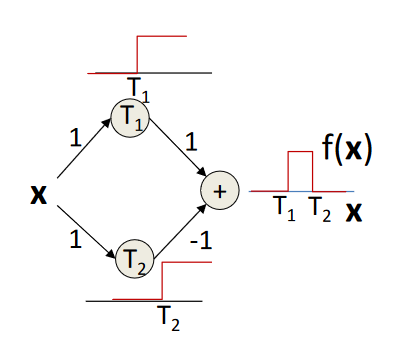
\includegraphics[width=0.5\textwidth]{1_3_unit_mlps}
\end{figure}

\begin{itemize}
	\item The input is a single scalar $\mathbf{x}$.
	\item The first neuron fires, meaning that the output becomes $1$ anytime the input $\mathbf{x}$ exceed the threshold value $T_1$.
	\item The second neuron also fires, meaning that the output becomes $1$ anytime the input $\mathbf{x}$ exceed the threshold value $T_2$.
	\item Their outputs are summed with values $1$ and $-1$ respectively.
	\item As $\mathbf{x}$ goes from large negative value to large positive value, assuming without loss of generality $T_1 < T_2$, eventually it will cross $T_1$ (At this point it has not yet crossed $T_2$).
	\item So at the first perceptron, the output is $1$ while it is still $0$ on the second perceptron.
	\item As we continue to increase $\mathbf{x}$, it will eventually crosses $T_2$ and the output of these 2 neurons will cancel out.
	\item The output of the overall circuit goes back to zero after passing $T_2$.
	\item This network will output $1$ if the input is between $T_1$ and $T_2$, and zero elsewhere.
\end{itemize}

\hfill\break
Suppose that we are given arbirary function as shown below:
\begin{figure}[H]
	\centering
	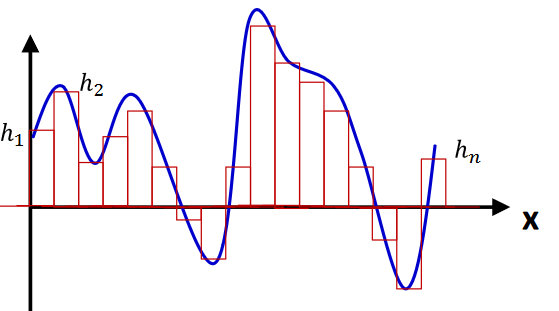
\includegraphics[width=0.5\textwidth]{1_arbitrary_continuous}
\end{figure}

\hfill\break
We can partition the input space into lots of little buckets (similar how ADC works), so that we can have one little subnet for each of the bucket. Then we can scale the outputs by the height of the function average within that range.

\begin{itemize}
	\item An MLP with many units can model an arbirary function over an input.
	\item We can get an arbirary precision by making the individual buckets smaller.
	\item This generalizes to functions of any number of inputs.
\end{itemize}

\subsection{Summary}
\begin{itemize}
	\item MLPs are connectionist computational models.
	\begin{itemize}
		\item Individual perceptrons are computational equivalent of neurons.
		\item The MLP is a layered composition of many perceptrons.
	\end{itemize}
		\item MLPs can model any Booleans function.
	\begin{itemize}
		\item Individual perceptrons can act as Boolean gates.
		\item Networks of perceptrons are Boolean gates.
		\item MLPs are universal Boolean functions.
	\end{itemize}
		\item MLPs can models any decision boundary.
	\begin{itemize}
		\item Individual perceptrons capture linear boundaries.
		\item Complex boundaries can be composed from the linear boundaries.
		\item MLPs can represent arbitrary decision boundaries.
		\item They can be used to classify data.
		\item MLPs are universal classifiers.
	\end{itemize}
\end{itemize}